\section{Background}
\label{sec:background}
\subsection{Bitcoin}

\textbf{Transaction} Transaction descibes the money flow from input addresses to output addresses. There are two popular ways to keep record in blockchain network. Account/Balance model is used in Ethereum, it is also the model we often encounter in our daily life, Bank, Paypal, etc, all implements such a model. Bitcoin, however, employs another model called UTXO, i.e. unspent transaction output. All of the unspent transactions are kept in each synchronized node. Figure\ref{fig:UTXO} illustrates the transaction flow in UTXO model. In this demonstration, user A got 10 bitcoin from mining, than A wants to send 5.5 of them to user B, so at first A's wallet is unlocked, and then 10 bitcoin is used as the input of the transaction, 5.5 bitcoin is sent to B, the remaining 4.5 bitcoin is sent back to A in the form of a newly created UTXO.
\begin{figure}[tbp]
\centerline{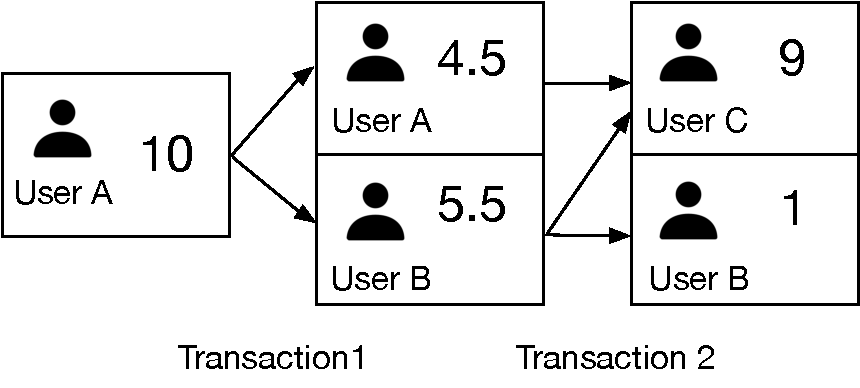
\includegraphics[width=0.8\columnwidth]{images/UTXO.pdf}}
\caption{The UTXO process}
\label{fig:UTXO}
\end{figure}

\textbf{Address}
Currently, there are three types of addresses in Bitcoin. The addresses are used to mark the input or output user in the Bitcoin transaction. When generating Bitcoin addresses, user should firstly generate a private key, then calculate the public key using this private key. Traditional bitcoin addresses derive directly from the public key, they are called Pay-to-Public-Key-Hash(P2PKH), this type of bitcoin addresses begin with the prefix 1. Anyone can send bitcoin to a P2PKH address, the UTXO that belongs to this address can only be spent by presenting the corresponding private key signature and public key hash. BIP0016\cite{BIP0016}, which was proposed in 2012 brought Pay-to-Script-Hash, this type of addresses are created from a transaction script, a typical application of this type of addresses is multi-signature transaction. It is also the most common implementation of P2SH function. This type of bitcoin addresses begin with the prefix 3. Besides, the segregated witness(SegWit) separate witness data in transaction inputs, which created bech32 addresses that begins with `bc1q'.

\subsection{Crowdsourcing Services}
Crowdsourcing service refers to obtaining work, information, opinions, etc., from people who submit their data via the internet. In the bitcoin community, crowdsourcing is a popular way to share and obtain information with each other in the community. It's also essential and important as the information linking the user and the bitcoin address is not available in decentralized platforms like blockchain. When crimes are conducted in centralized financial service such as banks, its easy to trace the criminals as the centralized services can provide. Decentralized services depend on crowdsourcing service to collect information. There are lots of famous crowdsourcing services, such as bitcointalk.org\cite{bitcointalk}, there are also submodule in discussion website like Reddit\cite{reddit}.
\subsection{Scams in Bitcoin}

Scam in bitcoin refers to fraudulent business or scheme that takes money or other goods from an unsuspected person. There has been different taxonomies towards bitcoin scams. Vasek et al \cite{vasek2015there} categorized scams into Ponzi schemes, mining scams, scam wallets and fradulent exchanges. However, new schemes continuously appear, and the distribution in scams varies a lot. The scammers usually appear in a group, that is for every scam group in reality, they may own a cluster of bitcoin addresses, there are money flows among these addresses.

\subsection{Bitcoin Clustering}
Concerning to secure the anonymity of bitcoin, bitcoin encourages using new addresses for each transactions to protect the privacy of users, but this increases the difficulty of linking addresses.
Bitcoin clustering aims at clustering bitcoin addresses that belong to the same entity. There are some heuristics proposed in recent years \cite{zhang2020heuristic}. And there are also software implementations based on these heuristics, or services for other use but implements clustering heuristics: GraphSense\cite{haslhofer2021graphsense}, BTCTester\cite{btctester}, BitcoinWhosWho\cite{bitcoinwhoswho}.
\subsection{Detection Based on ML and Neural Network}
 
 Graph neural network is a class of neural networks for processing data represented by graph data structures. Various graph neural network structures have been proposed in these years, such as Graph Convolutional Network\cite{kipf2016semi}, Graph Attention Network\cite{velivckovic2017graph}. As bitcoin addresses are linked by transactions, there are a lot of graph features to explorer. Traditional machine learning methods are implemented to compare with the graph neural network methods.


